\documentclass[]{article}
\usepackage{lmodern}
\usepackage{amssymb,amsmath}
\usepackage{ifxetex,ifluatex}
\usepackage{fixltx2e} % provides \textsubscript
\ifnum 0\ifxetex 1\fi\ifluatex 1\fi=0 % if pdftex
  \usepackage[T1]{fontenc}
  \usepackage[utf8]{inputenc}
\else % if luatex or xelatex
  \ifxetex
    \usepackage{mathspec}
  \else
    \usepackage{fontspec}
  \fi
  \defaultfontfeatures{Ligatures=TeX,Scale=MatchLowercase}
\fi
% use upquote if available, for straight quotes in verbatim environments
\IfFileExists{upquote.sty}{\usepackage{upquote}}{}
% use microtype if available
\IfFileExists{microtype.sty}{%
\usepackage{microtype}
\UseMicrotypeSet[protrusion]{basicmath} % disable protrusion for tt fonts
}{}
\usepackage[margin=1in]{geometry}
\usepackage{hyperref}
\hypersetup{unicode=true,
            pdfborder={0 0 0},
            breaklinks=true}
\urlstyle{same}  % don't use monospace font for urls
\usepackage{natbib}
\bibliographystyle{plainnat}
\usepackage{color}
\usepackage{fancyvrb}
\newcommand{\VerbBar}{|}
\newcommand{\VERB}{\Verb[commandchars=\\\{\}]}
\DefineVerbatimEnvironment{Highlighting}{Verbatim}{commandchars=\\\{\}}
% Add ',fontsize=\small' for more characters per line
\usepackage{framed}
\definecolor{shadecolor}{RGB}{248,248,248}
\newenvironment{Shaded}{\begin{snugshade}}{\end{snugshade}}
\newcommand{\KeywordTok}[1]{\textcolor[rgb]{0.13,0.29,0.53}{\textbf{{#1}}}}
\newcommand{\DataTypeTok}[1]{\textcolor[rgb]{0.13,0.29,0.53}{{#1}}}
\newcommand{\DecValTok}[1]{\textcolor[rgb]{0.00,0.00,0.81}{{#1}}}
\newcommand{\BaseNTok}[1]{\textcolor[rgb]{0.00,0.00,0.81}{{#1}}}
\newcommand{\FloatTok}[1]{\textcolor[rgb]{0.00,0.00,0.81}{{#1}}}
\newcommand{\ConstantTok}[1]{\textcolor[rgb]{0.00,0.00,0.00}{{#1}}}
\newcommand{\CharTok}[1]{\textcolor[rgb]{0.31,0.60,0.02}{{#1}}}
\newcommand{\SpecialCharTok}[1]{\textcolor[rgb]{0.00,0.00,0.00}{{#1}}}
\newcommand{\StringTok}[1]{\textcolor[rgb]{0.31,0.60,0.02}{{#1}}}
\newcommand{\VerbatimStringTok}[1]{\textcolor[rgb]{0.31,0.60,0.02}{{#1}}}
\newcommand{\SpecialStringTok}[1]{\textcolor[rgb]{0.31,0.60,0.02}{{#1}}}
\newcommand{\ImportTok}[1]{{#1}}
\newcommand{\CommentTok}[1]{\textcolor[rgb]{0.56,0.35,0.01}{\textit{{#1}}}}
\newcommand{\DocumentationTok}[1]{\textcolor[rgb]{0.56,0.35,0.01}{\textbf{\textit{{#1}}}}}
\newcommand{\AnnotationTok}[1]{\textcolor[rgb]{0.56,0.35,0.01}{\textbf{\textit{{#1}}}}}
\newcommand{\CommentVarTok}[1]{\textcolor[rgb]{0.56,0.35,0.01}{\textbf{\textit{{#1}}}}}
\newcommand{\OtherTok}[1]{\textcolor[rgb]{0.56,0.35,0.01}{{#1}}}
\newcommand{\FunctionTok}[1]{\textcolor[rgb]{0.00,0.00,0.00}{{#1}}}
\newcommand{\VariableTok}[1]{\textcolor[rgb]{0.00,0.00,0.00}{{#1}}}
\newcommand{\ControlFlowTok}[1]{\textcolor[rgb]{0.13,0.29,0.53}{\textbf{{#1}}}}
\newcommand{\OperatorTok}[1]{\textcolor[rgb]{0.81,0.36,0.00}{\textbf{{#1}}}}
\newcommand{\BuiltInTok}[1]{{#1}}
\newcommand{\ExtensionTok}[1]{{#1}}
\newcommand{\PreprocessorTok}[1]{\textcolor[rgb]{0.56,0.35,0.01}{\textit{{#1}}}}
\newcommand{\AttributeTok}[1]{\textcolor[rgb]{0.77,0.63,0.00}{{#1}}}
\newcommand{\RegionMarkerTok}[1]{{#1}}
\newcommand{\InformationTok}[1]{\textcolor[rgb]{0.56,0.35,0.01}{\textbf{\textit{{#1}}}}}
\newcommand{\WarningTok}[1]{\textcolor[rgb]{0.56,0.35,0.01}{\textbf{\textit{{#1}}}}}
\newcommand{\AlertTok}[1]{\textcolor[rgb]{0.94,0.16,0.16}{{#1}}}
\newcommand{\ErrorTok}[1]{\textcolor[rgb]{0.64,0.00,0.00}{\textbf{{#1}}}}
\newcommand{\NormalTok}[1]{{#1}}
\usepackage{graphicx,grffile}
\makeatletter
\def\maxwidth{\ifdim\Gin@nat@width>\linewidth\linewidth\else\Gin@nat@width\fi}
\def\maxheight{\ifdim\Gin@nat@height>\textheight\textheight\else\Gin@nat@height\fi}
\makeatother
% Scale images if necessary, so that they will not overflow the page
% margins by default, and it is still possible to overwrite the defaults
% using explicit options in \includegraphics[width, height, ...]{}
\setkeys{Gin}{width=\maxwidth,height=\maxheight,keepaspectratio}
\IfFileExists{parskip.sty}{%
\usepackage{parskip}
}{% else
\setlength{\parindent}{0pt}
\setlength{\parskip}{6pt plus 2pt minus 1pt}
}
\setlength{\emergencystretch}{3em}  % prevent overfull lines
\providecommand{\tightlist}{%
  \setlength{\itemsep}{0pt}\setlength{\parskip}{0pt}}
\setcounter{secnumdepth}{0}
% Redefines (sub)paragraphs to behave more like sections
\ifx\paragraph\undefined\else
\let\oldparagraph\paragraph
\renewcommand{\paragraph}[1]{\oldparagraph{#1}\mbox{}}
\fi
\ifx\subparagraph\undefined\else
\let\oldsubparagraph\subparagraph
\renewcommand{\subparagraph}[1]{\oldsubparagraph{#1}\mbox{}}
\fi

%%% Use protect on footnotes to avoid problems with footnotes in titles
\let\rmarkdownfootnote\footnote%
\def\footnote{\protect\rmarkdownfootnote}

%%% Change title format to be more compact
\usepackage{titling}

% Create subtitle command for use in maketitle
\newcommand{\subtitle}[1]{
  \posttitle{
    \begin{center}\large#1\end{center}
    }
}

\setlength{\droptitle}{-2em}
  \title{}
  \pretitle{\vspace{\droptitle}}
  \posttitle{}
  \author{}
  \preauthor{}\postauthor{}
  \date{}
  \predate{}\postdate{}


\begin{document}

\subsection{Packages used in the
exploration}\label{packages-used-in-the-exploration}

We will be using the packages listed below over the course of the
experiments.

\begin{Shaded}
\begin{Highlighting}[]
\KeywordTok{library}\NormalTok{(purrr)}
\KeywordTok{library}\NormalTok{(magrittr)}
\KeywordTok{library}\NormalTok{(rts)}
\KeywordTok{library}\NormalTok{(depmixS4)}
\KeywordTok{library}\NormalTok{(TTR)}
\KeywordTok{library}\NormalTok{(ggplot2)}
\KeywordTok{library}\NormalTok{(reshape2)}
\KeywordTok{library}\NormalTok{(gridExtra)}
\KeywordTok{library}\NormalTok{(dplyr)}
\KeywordTok{library}\NormalTok{(ggplot2)}
\KeywordTok{library}\NormalTok{(tidyr)}
\KeywordTok{library}\NormalTok{(lubridate)}
\KeywordTok{library}\NormalTok{(KMsurv)}
\KeywordTok{library}\NormalTok{(tibble)}
\KeywordTok{library}\NormalTok{(stringr)}
\KeywordTok{library}\NormalTok{(tidyr)}
\end{Highlighting}
\end{Shaded}

\subsection{The evolution of terrorism over time (year and month) by
region and world wide
figures}\label{the-evolution-of-terrorism-over-time-year-and-month-by-region-and-world-wide-figures}

Plotting the monthly totals of deaths due to terrorism by region and by
world wide figures,we see using these two plots , temporal, regional and
regional-temproal relationships emerge. The relationships are shown
below:

\begin{enumerate}
\def\labelenumi{\arabic{enumi}.}
\item
  Since records have started to be recorded in 1970, deaths due
  terrorism is on the rise. From the time series world plot we see that
  during the 1980's there was a sharp rise in terrorism. This flattened
  out with end of the cold war and appears to be declining up to the end
  of 1990's, after September the 11th 2001 there is an increase in
  terrorism. This increases dramtically with the invasions of Iraq and
  Afganistan, it increases upto 2007, before sharply rising after 2010.
\item
  When examining the time series plot by month by region, We see a more
  refined pattern. We can see the spike in terrorism in the 1980's due
  to a sharp rise in terrorism in Central America and later in the
  decade in South America. This fell at the end of the 1980's and start
  of the 1990's. Terrorism fell accross all regions before beginning to
  rise in the 2000's especially in sub-saharan Africa, the middle east
  and North africa and south Asia (particularly Afganistan and
  Pakistan).
\end{enumerate}

The time series plot for the different regions is shown below. The
temporal, regional relationships described above are clearly visible.

\includegraphics{Peters_experiment_markdown_files/figure-latex/unnamed-chunk-2-1.pdf}

While the world wide time series plot quite clearly shows the rise in
terrorism worlwide since 1970. Plotting by region again the specific
temporal regional relationships are clearly visible, these are the sharp
rise in the 1980's to the start of the 1990's of deaths due to
terrorism. Again a regional shift of deaths due to terrorism has shifted
to the Middle East, this rose after the September 11th attacks and the
subsequent invasions of Afganistan and Pakistan.

\includegraphics{Peters_experiment_markdown_files/figure-latex/unnamed-chunk-3-1.pdf}

\subsection{Data displayed as time series by
Year}\label{data-displayed-as-time-series-by-year}

Similarly we can see the global rise in deaths due terrorism by year
since 1970, using a year interval instead of month interval (which was
used in the previous plots) . The pattern is even more clearer the time
series of deaths by years and deaths by year and region is plotted. The
below shot shows the number of deaths globally (not broken out by
region). We see a rise in the late 1970's and 1980's which persisted
till 2010 followed by a large increase thereafter.

\includegraphics{Peters_experiment_markdown_files/figure-latex/unnamed-chunk-4-1.pdf}

Now by year and region. A clear pattern emerges the rise in number of
deaths due to terrorism in Central America in the 1980's which fell
sharply towards the end of the cold war A rise in terrorism is also seen
in the

\includegraphics{Peters_experiment_markdown_files/figure-latex/unnamed-chunk-5-1.pdf}

\subsection{Viewing deaths by region and year using stacked bar
charts}\label{viewing-deaths-by-region-and-year-using-stacked-bar-charts}

Now lets look at the data as a stacked bar chart. The stacked bar chart
lets us assess the contributing fraction of total deaths for a
particular time interval.When viewed as a stacked bar plot (with the
region represented as portion of the bar). It is clear to see the fall
off in terrororism in South America and Central America, corresponding
with a rise in deaths due to terrorism in the Middle East and south
Asia. For the last decade the number of deaths that are due to terrorism
has been dominated by South Asia, the Middle East and Sub Saharan
Africa.

\includegraphics{Peters_experiment_markdown_files/figure-latex/unnamed-chunk-6-1.pdf}

\subsection{Viewing deaths by attack vector
type}\label{viewing-deaths-by-attack-vector-type}

Examining the plot of deaths due to attack vector (Armed assault,
Hijacking, Hostage aking etc) is shown below. Again a temporal
relationship exists with since the emergence of bominbgs and explosives
as the prominent attack vector. Also the emergence of Hostage taking
(Barricade incidents and Kidnapping).

\begin{verbatim}
## 'data.frame':    398 obs. of  3 variables:
##  $ iyear          : int  1970 1970 1970 1970 1970 1970 1970 1970 1970 1971 ...
##  $ attacktype1_txt: Factor w/ 9 levels "Armed Assault",..: 1 2 3 4 5 6 7 8 9 1 ...
##  $ num_of_killed  : num  36 15 96 9 1 0 10 0 4 14 ...
\end{verbatim}

\includegraphics{Peters_experiment_markdown_files/figure-latex/unnamed-chunk-7-1.pdf}

A similar trend is observed when we just look at the Middle east, with
Bombings and exlosions the attack vector that is dominating.

\includegraphics{Peters_experiment_markdown_files/figure-latex/unnamed-chunk-8-1.pdf}

\subsection{Viewing deaths by Weapon
type}\label{viewing-deaths-by-weapon-type}

Plotting the data as a stacked bar plot shows similar results to the
plot of the stacked bar plot by year of counts of attacks by attack
vector.

\includegraphics{Peters_experiment_markdown_files/figure-latex/unnamed-chunk-9-1.pdf}

Looking at just the middle east again we see similar results to the plot
of vector type

\subsection{Viewing deaths by group for countries in the middle east
using stacked bar
charts}\label{viewing-deaths-by-group-for-countries-in-the-middle-east-using-stacked-bar-charts}

\subsection{Viewing deaths by countries in the middle east using stacked
bar
charts}\label{viewing-deaths-by-countries-in-the-middle-east-using-stacked-bar-charts}

Plotting the deaths of those killed from terrorism it's quite clear that
terrorism was really not a concern until after the invasion in 2003.

\includegraphics{Peters_experiment_markdown_files/figure-latex/unnamed-chunk-11-1.pdf}

\subsection{Examining the number of deaths by
type.}\label{examining-the-number-of-deaths-by-type.}

Syria shows a similar pattern there was a small outbreak of terrorism in
1981 due to the muslim brotherhood rising in 1981.

\includegraphics{Peters_experiment_markdown_files/figure-latex/unnamed-chunk-12-1.pdf}

Looking at Lebanon we can see the deaths due to the cicl war in the
1970's and 1980's however there does apear to be a year on year rise in
deaths due to terrorism at the tailend of 2000's.

\includegraphics{Peters_experiment_markdown_files/figure-latex/unnamed-chunk-13-1.pdf}
Similarly Turkey has seen a rise in deaths due to terrorism since the
arab spring.

\includegraphics{Peters_experiment_markdown_files/figure-latex/unnamed-chunk-14-1.pdf}
\#\# Stacked bar plot of counts of deaths by year by country for the
middle east

From looking at the whole middle east the number of deaths due to
terrorism are increasing and are made up predominatly of fatalities from
Iraq, Syria and Yemen.

\includegraphics{Peters_experiment_markdown_files/figure-latex/unnamed-chunk-15-1.pdf}

Looking at the average killed per incident per year for Iraq since 2000
we can see a peak around 2007 a fall and then a steady increase since
2011.

\includegraphics{Peters_experiment_markdown_files/figure-latex/unnamed-chunk-16-1.pdf}
The daily number of deaths in Iraq due to terrorism since 1975

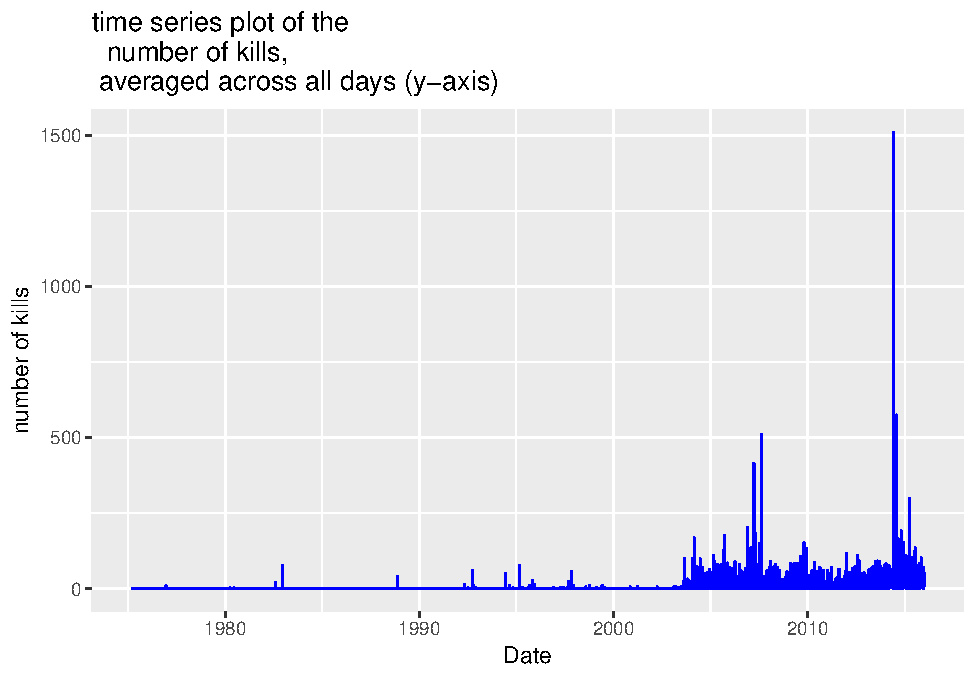
\includegraphics{Peters_experiment_markdown_files/figure-latex/unnamed-chunk-17-1.pdf}

The daily counts are really interesting as we may be able to model this
data using some preliminary methods to get a sense of when the changes
and what were the covariates of these events. To do this we use a two
techniques Poisson Regression and Hidden markov Models: (a) The poisson
model as we are modelling count data might be effective at modelling the
numbers of dead killed per month and seeing if the different events that
took place specifically interventions have an effect on lowering or
increasing the death toll due to terrorism. (b) Hidden Markov Model
might be useful at modelling the transition of Iraq from an era of
realtive peace(low numbers of attack) to era's with high number of
terrorist attacks. This change in state from an era of peace to that of
outright insurgency would ve very usefull to look at to examine when a
particular change occurred. But also from a point of view if seeing if
interventions had an effect and when after an intervention.

\subsection{Poisson regession}\label{poisson-regession}

We build a poisson model and a quasi-poisson model, the quasi-poisson
model is used as overdispersion of our data is observed in the poisson
model. The quasi poisson model did not seem to resolve this issue. But
we can see that from the summary table that the Periodsurge,
Period,Pre\_invasion. We create a categorical variable to describe the
period, these are:

\begin{enumerate}
\def\labelenumi{\arabic{enumi}.}
\tightlist
\item
  ``01/05/2003'', Period=Pre Invasion
\item
  ``01/05/2003'' to ``01/01/2007'', Period =Post\_Invasion
\item
  ``01/01/2007'' to ``31/12/2007'', Period =Surge
\item
  ``01/01/2008'' to ``31/12/2009'', Period =Post Surge
\item
  ``01/01/2008'' to ``31/12/2009'', Period =Drawdown
\item
  ``01/01/2010'' to ``31/12/2012'', Period =Pullout
\item
  after ``31/12/2012'', Period = PostPullout
\end{enumerate}

From the poisson model we can see the residual deviance is lower than
the null deviance, however the model does not explain the deviance very
well. We do not learn alot from this experiment except that the surge
had a positive effect (increased the number killed) on the number of
people killed. While the pullout (the period after the surge) saw a
significant drop in the number of people killed due to terrorism.

\begin{verbatim}
## 
## Call:
## glm(formula = kills_sum ~ ., family = "poisson", data = iraq.kills.summary.period)
## 
## Deviance Residuals: 
##     Min       1Q   Median       3Q      Max  
## -19.415   -4.219   -1.867    2.302   71.652  
## 
## Coefficients:
##                       Estimate Std. Error z value Pr(>|z|)    
## (Intercept)          1.4566812  0.1429542   10.19   <2e-16 ***
## month_since_1970     0.0097591  0.0003505   27.84   <2e-16 ***
## PeriodPost_Invasion  0.5147116  0.0228935   22.48   <2e-16 ***
## PeriodPostPullout    0.6263933  0.0276487   22.66   <2e-16 ***
## PeriodPre_Invasion  -1.8482094  0.0635771  -29.07   <2e-16 ***
## PeriodPullout       -0.5031853  0.0212600  -23.67   <2e-16 ***
## PeriodSurge          1.0782566  0.0194152   55.54   <2e-16 ***
## ---
## Signif. codes:  0 '***' 0.001 '**' 0.01 '*' 0.05 '.' 0.1 ' ' 1
## 
## (Dispersion parameter for poisson family taken to be 1)
## 
##     Null deviance: 94293  on 251  degrees of freedom
## Residual deviance: 18048  on 245  degrees of freedom
## AIC: 19401
## 
## Number of Fisher Scoring iterations: 6
\end{verbatim}

\begin{verbatim}
## 
## Call:
## glm(formula = kills_sum ~ ., family = "quasipoisson", data = iraq.kills.summary.period)
## 
## Deviance Residuals: 
##     Min       1Q   Median       3Q      Max  
## -19.415   -4.219   -1.867    2.302   71.652  
## 
## Coefficients:
##                      Estimate Std. Error t value Pr(>|t|)    
## (Intercept)          1.456681   1.500151   0.971  0.33249    
## month_since_1970     0.009759   0.003678   2.653  0.00850 ** 
## PeriodPost_Invasion  0.514712   0.240242   2.142  0.03314 *  
## PeriodPostPullout    0.626393   0.290143   2.159  0.03183 *  
## PeriodPre_Invasion  -1.848209   0.667174  -2.770  0.00603 ** 
## PeriodPullout       -0.503185   0.223101  -2.255  0.02499 *  
## PeriodSurge          1.078257   0.203742   5.292 2.68e-07 ***
## ---
## Signif. codes:  0 '***' 0.001 '**' 0.01 '*' 0.05 '.' 0.1 ' ' 1
## 
## (Dispersion parameter for quasipoisson family taken to be 110.1226)
## 
##     Null deviance: 94293  on 251  degrees of freedom
## Residual deviance: 18048  on 245  degrees of freedom
## AIC: NA
## 
## Number of Fisher Scoring iterations: 6
\end{verbatim}

The plot of the predicted versus the actuals is shown below:

\includegraphics{Peters_experiment_markdown_files/figure-latex/unnamed-chunk-19-1.pdf}

As we are seeing an increase incounts of deaths over time it may make
sense to model this as a quadratic effect we do this below and we see
and plot the results, doing so we see from the graph no better fit and
also the model remins massively overdispersed.

\includegraphics{Peters_experiment_markdown_files/figure-latex/unnamed-chunk-20-1.pdf}

\begin{verbatim}
## 
## Call:
## glm(formula = kills_sum ~ ., family = "quasipoisson", data = iraq.kills.summary.period)
## 
## Deviance Residuals: 
##     Min       1Q   Median       3Q      Max  
## -19.415   -4.219   -1.867    2.302   71.652  
## 
## Coefficients:
##                      Estimate Std. Error t value Pr(>|t|)    
## (Intercept)          1.456681   1.500151   0.971  0.33249    
## month_since_1970     0.009759   0.003678   2.653  0.00850 ** 
## PeriodPost_Invasion  0.514712   0.240242   2.142  0.03314 *  
## PeriodPostPullout    0.626393   0.290143   2.159  0.03183 *  
## PeriodPre_Invasion  -1.848209   0.667174  -2.770  0.00603 ** 
## PeriodPullout       -0.503185   0.223101  -2.255  0.02499 *  
## PeriodSurge          1.078257   0.203742   5.292 2.68e-07 ***
## ---
## Signif. codes:  0 '***' 0.001 '**' 0.01 '*' 0.05 '.' 0.1 ' ' 1
## 
## (Dispersion parameter for quasipoisson family taken to be 110.1226)
## 
##     Null deviance: 94293  on 251  degrees of freedom
## Residual deviance: 18048  on 245  degrees of freedom
## AIC: NA
## 
## Number of Fisher Scoring iterations: 6
\end{verbatim}

The summary of the poisson model is shown below:

\begin{verbatim}
## 
## Call:
## glm(formula = kills_sum ~ ., family = "quasipoisson", data = iraq.kills.summary.period)
## 
## Deviance Residuals: 
##     Min       1Q   Median       3Q      Max  
## -19.415   -4.219   -1.867    2.302   71.652  
## 
## Coefficients:
##                      Estimate Std. Error t value Pr(>|t|)    
## (Intercept)          1.456681   1.500151   0.971  0.33249    
## month_since_1970     0.009759   0.003678   2.653  0.00850 ** 
## PeriodPost_Invasion  0.514712   0.240242   2.142  0.03314 *  
## PeriodPostPullout    0.626393   0.290143   2.159  0.03183 *  
## PeriodPre_Invasion  -1.848209   0.667174  -2.770  0.00603 ** 
## PeriodPullout       -0.503185   0.223101  -2.255  0.02499 *  
## PeriodSurge          1.078257   0.203742   5.292 2.68e-07 ***
## ---
## Signif. codes:  0 '***' 0.001 '**' 0.01 '*' 0.05 '.' 0.1 ' ' 1
## 
## (Dispersion parameter for quasipoisson family taken to be 110.1226)
## 
##     Null deviance: 94293  on 251  degrees of freedom
## Residual deviance: 18048  on 245  degrees of freedom
## AIC: NA
## 
## Number of Fisher Scoring iterations: 6
\end{verbatim}

\subsection{Hiden Markov Models}\label{hiden-markov-models}

Hidden markov models are often used to model for time regime detection
and shifts in these regimes. HMM's are a probalistic process which
examine the current state along a timeline to make a prediction about
the next state. We use a two state and a three state HMM to model.

The two state model output is shown below. the summary of the model
output can be seen.

\begin{verbatim}
## iteration 0 logLik: -16666.39 
## iteration 5 logLik: -14811.46 
## iteration 10 logLik: -14696.15 
## iteration 15 logLik: -14667.42 
## iteration 20 logLik: -14660.45 
## iteration 25 logLik: -14658.61 
## iteration 30 logLik: -14658.13 
## iteration 35 logLik: -14658.01 
## iteration 40 logLik: -14657.99 
## iteration 45 logLik: -14657.98 
## iteration 50 logLik: -14657.98 
## converged at iteration 51 with logLik: -14657.98
\end{verbatim}

\begin{verbatim}
## Response parameters 
## Resp 1 : gaussian 
##     Re1.(Intercept) Re1.sd
## St1          28.377 30.337
## St2           2.654  2.774
\end{verbatim}

\begin{verbatim}
##   state         S1        S2
## 1     2 0.00000000 1.0000000
## 2     2 0.48370298 0.5162970
## 3     2 0.06537087 0.9346291
## 4     2 0.02324131 0.9767587
## 5     2 0.02614839 0.9738516
## 6     2 0.03331867 0.9666813
\end{verbatim}

\begin{verbatim}
##        idate sum_kill
## 1 1975-03-01        0
## 2 1976-12-15       10
## 3 1976-12-18        0
## 4 1976-12-24        2
## 5 1979-06-15        1
## 6 1979-11-21        0
\end{verbatim}

\begin{verbatim}
## [1] 3829
\end{verbatim}

\begin{verbatim}
## [1] 3829
\end{verbatim}

\begin{verbatim}
## 1 2 3 4 5 6 
## 1 1 1 1 1 1
\end{verbatim}

we now plot the data to get an idea of the times were

\bibliography{sample}


\end{document}
